\section{Readout Electronic Design}
\label{sec:electronic_design}
The design of the readout electronics depends mainly on the directionality radiation sensor (see sec. \ref{sec:radiation_sensor}) and the ASIC VATA466 (see \cite{Meier2016VATA466}) architecture and drive requirements.
The sensor needs a high voltage supply (see sec. \ref{sec:hv_supply}) to create a reverse bias, the ASIC (see sec. \ref{sec:vata466_baseboard}) is used to readout the sensor data.
The ASIC itself demands some stable supply voltages (see sec. \ref{sec:power_supplies}) and a bias current (see sec. \ref{sec:bias_current}).
To have access to the spectroscopic mode for configuration purposes an ADC (Analog Digital Converter) is needed (see sec. \ref{sec:adc}).
Finally the power and data have to be interfaced with the rest of the cubesat (see sec. \ref{sec:interface_cubesat}).
The block diagram in fig. \ref{fig:electronic_block_diagram} shows the relationship between the different functional blocks of this electronic system.
\begin{figure}[H]
    \centering
    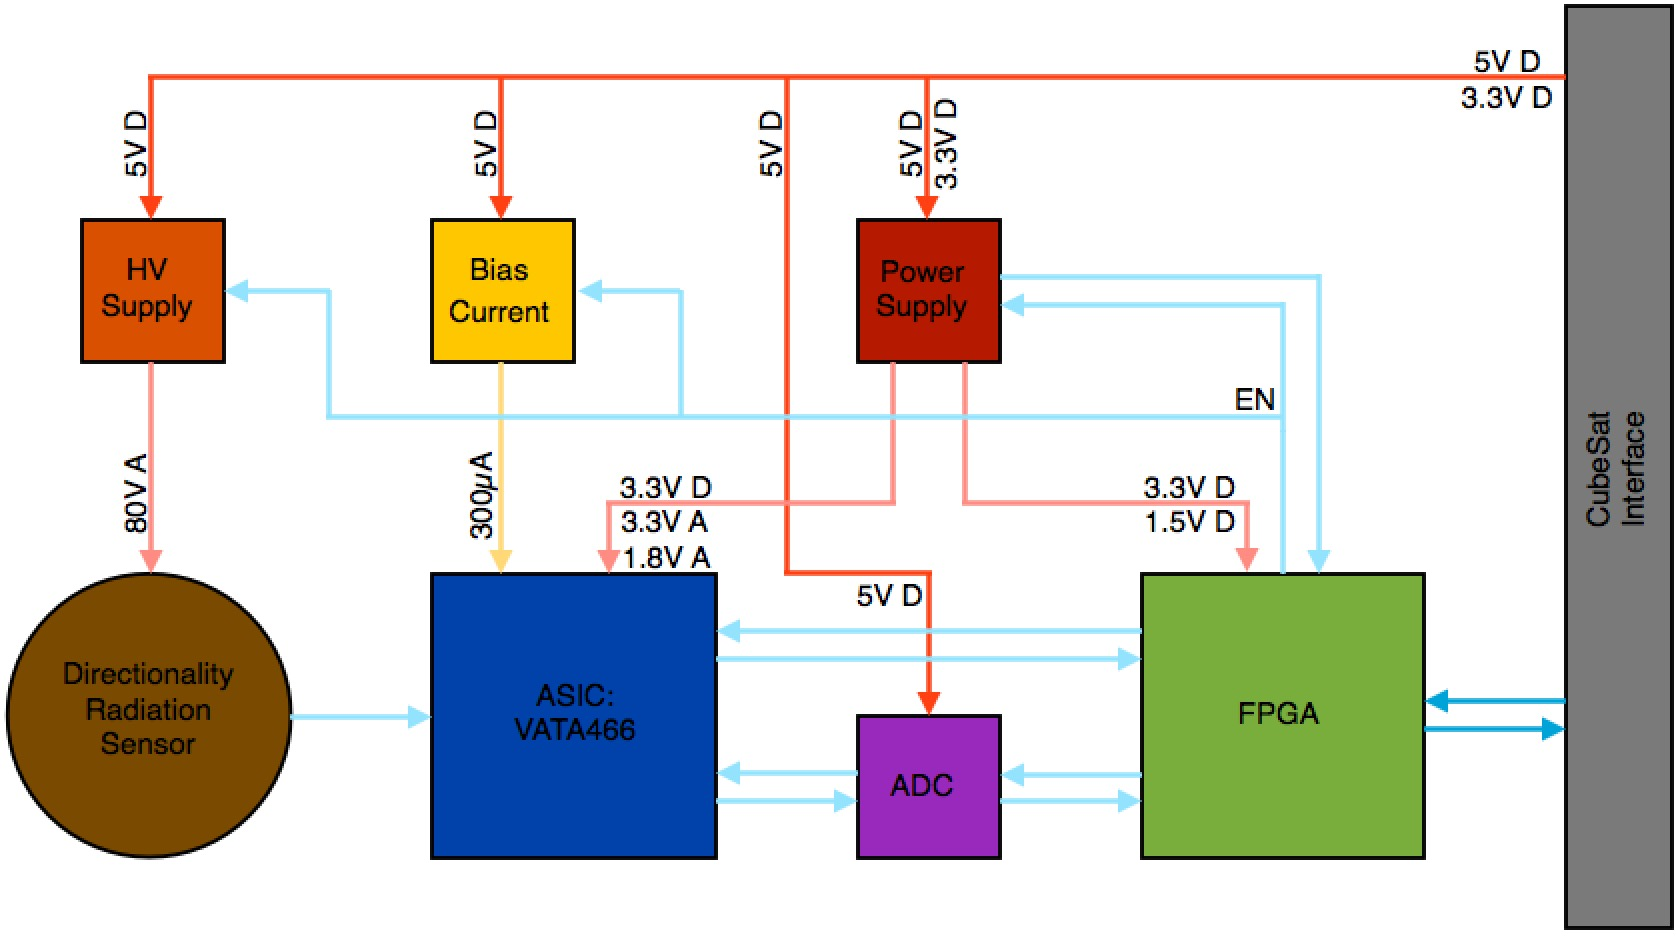
\includegraphics[width=1\textwidth]{electronic_block_diagram.jpg}
    \caption[Block Diagram Readout Electronics]{Block diagram of directional radiation sensor's readout electronics. \\    (Power: Red Arrows; Data: Blue Arrows)}
    \label{fig:electronic_block_diagram}
\end{figure}

The design has to be optimized in terms of power consumption, size and radiation hardness. 
For the latter it was discussed with PSI that the final design could be tested for it's radiation resistance and therefore much cheaper and not officially radiation hardened components can be chosen.
Size and power considerations mainly have to be traded-off against signal quality.
It is important to stay in the boundaries given by the data sheet of the ASIC to ensure a correct functioning of the instrument.


\subsection{VATA466 Baseboard}
\label{sec:vata466_baseboard}
The schematic ``VATA466\_Base\_Board.SchDoc'' includes all the basic building blocks of the electronic design and therefore resembles largely to the block diagram and description in sec. \ref{sec:electronic_design}.
A data bus connects all the command and data lines between the different modules and the FPGA.
A power bus distributes the correct voltages to the specific systems.

\subsubsection{ASIC: VATA466}
\label{sec:asic}
In the schematic ``VATA466.SchDoc'' the ASIC is divided into his functional subparts.
Figure \ref{fig:signals_pads} shows a schematic representation of the ASIC's functions and pins.
\begin{figure}[H]
    \centering
    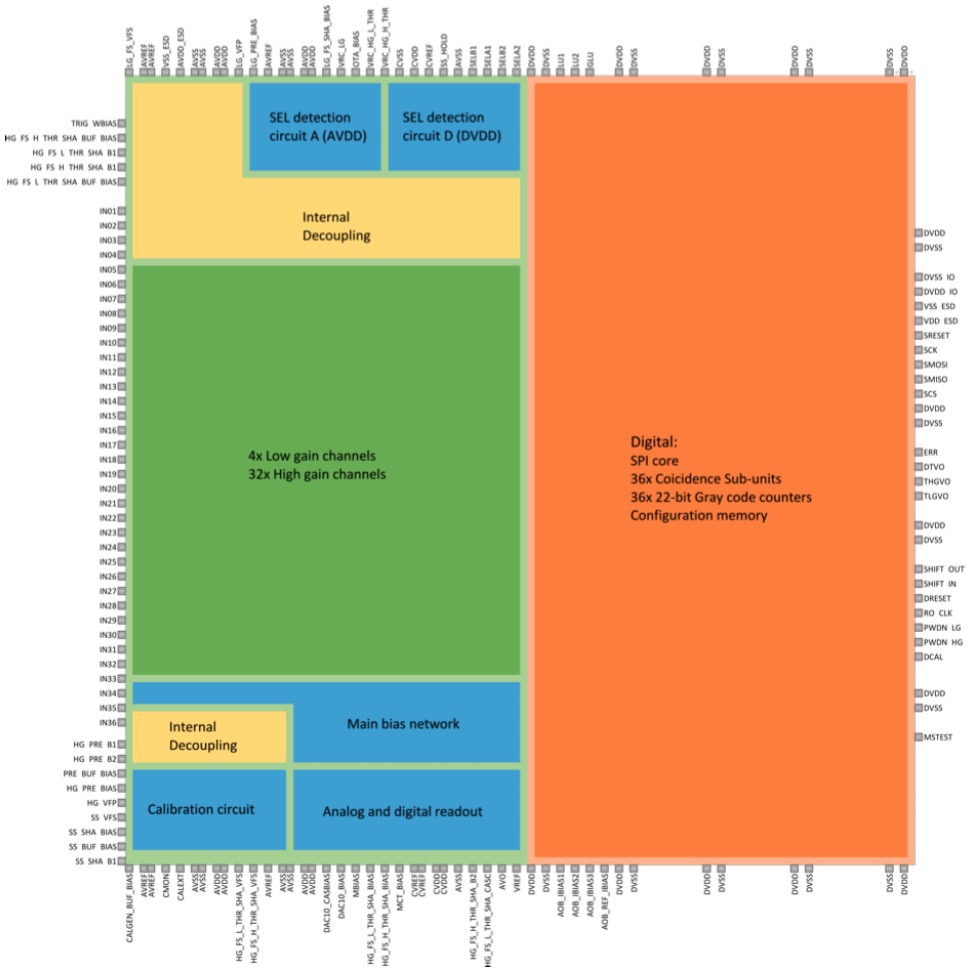
\includegraphics[width=0.7\textwidth]{signals_pads_chip.jpg}
    \caption[Signals and Chip Pad Frame]{Schematic overview of subparts and pins of the ASIC.\cite[p. 14, fig. 3]{Meier2016VATA466}}
    \label{fig:signals_pads}
\end{figure}

There are 36 CSA (charge sensitive pre-amplifiers), called U19A in the schematics, 4 of them have a low gain and 32 a high gain.
The DRS has 31 detector diodes and therefore uses 31 inputs of the high gain channels.

The ASIC also contains two power subparts, an analogue one (U19B) and a digital one (U19C).
They differ in that the analogue input voltages have strict requirements and need to have low noise since they are going to interact directly with the signals in the ASIC.
The digital input voltage is only used for the logic in the ASIC and is therefore less critical.
These inputs should be strictly isolated to avoid any degradation of the measurements.
The supply voltages will be discussed in more detail in section \ref{sec:power_supplies}.

The next subunit of the ASIC holds all his bias and test-pads (U19D).
The bias network will be described in more detail in section \ref{sec:bias_current}.
The test-pads can be used to debug the ASIC and to directly readout some of it's internal signals.
The following table describes the pins purposes and gives recommendations for external decoupling:
\begin{table}[h!]
	\centering
    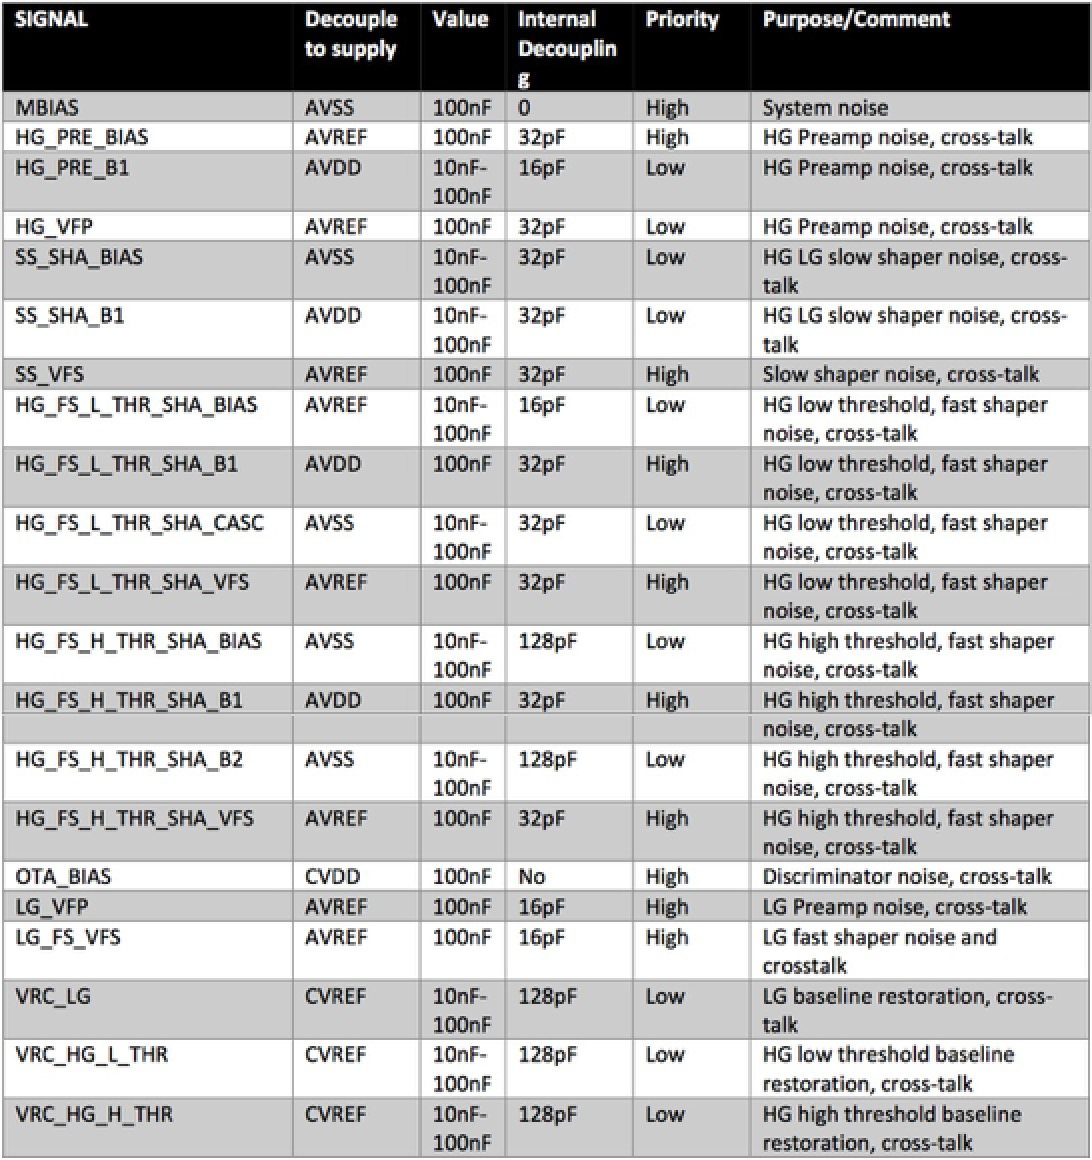
\includegraphics[width=0.7\textwidth]{test-pins.jpg}
    \caption[Test-pins Purpose and External Decoupling]{Purposes of the different test-pins and recoomendations for external decoupling.\cite[p. 65, tab. 31]{Meier2016VATA466}}
	\label{tab:test-pads}
\end{table}

The last subpart of the ASIC regroups all pins used for the readout and commands (U19E).
It uses SPI (Serial Peripheral Interface) to read or write over the ASIC's registers and thereby enables the use of the counting mode.
A calibration subunit can be used to test and calibrate the gain in the pre-amplifier, slow shapers and trigger the increment of a counter in a channel.
The power down block is used to power down the 4 low gain channels (1 to 4) and\/or 16 high gain channels (21 to 36), channels 5 to 20 are always powered on.
A single analogue output is provided through the AVO pin, which allows the readout of the pulse heights from all channels via multiplexing (see sec. \ref{sec:adc}).
The multiplexer is controlled through the A\&D channel readout block and is therefore used to setup the spectroscopic mode of the ASIC.
The trigger out block is used to indicate the triggering of either a low-gain or high-gain channel or the digital multiplexer.
The last block enables the latch-up detection in the ASIC and will be further explained in the next section.\cite{Meier2016VATA466}

\subsubsection{Latch-up Detector}
\label{sec:latchup_detector}
There are two latch-up detection modules included in the ASIC.
They each have two inputs SELA and SELB and one output LU.
A global latch-up signal (GLU) is created through a logic OR between the two latch-up detector outputs.
The schematic ``Latch\_Up\_Power.SchDoc'' represents an implementation of the recommended external circuit (see fig. \ref{fig:latch-up}).
\begin{figure}[H]
    \centering
    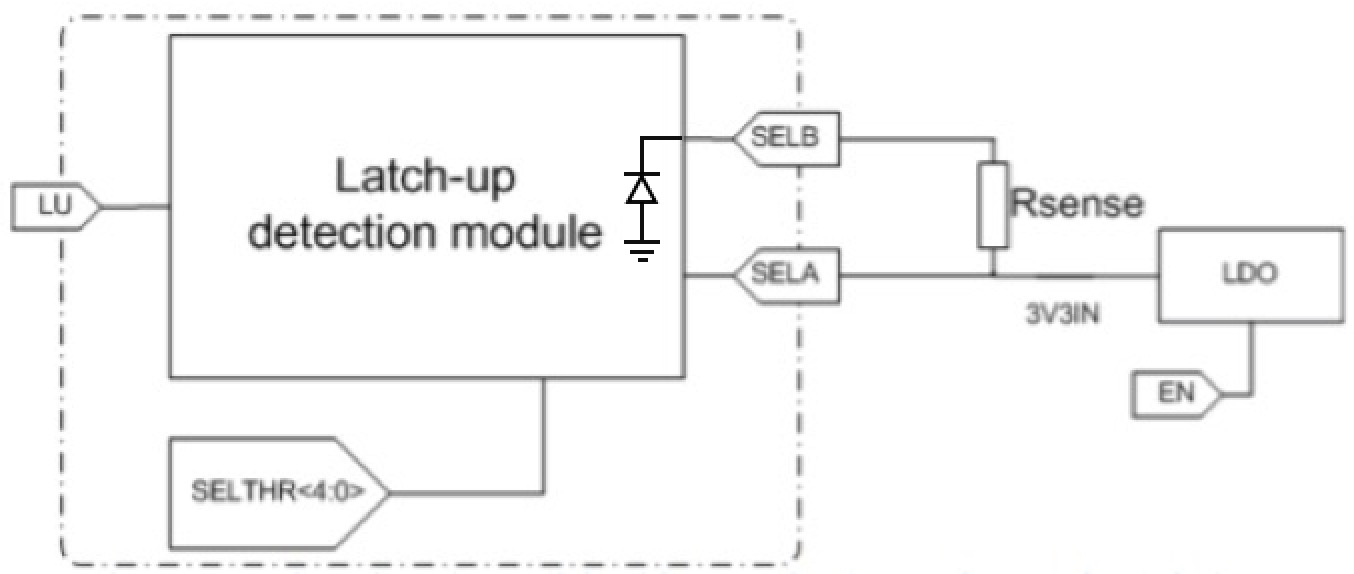
\includegraphics[width=0.6\textwidth]{latch-up.jpg}
    \caption[Latch-up Detection Module]{Reference design of an external latch-up detection circuit.\cite[p. 66, fig. 12]{Meier2016VATA466}}
    \label{fig:latch-up}
\end{figure}

The circuit consists of a LDO (U7 \& U8\footnote{LT1763}) which provide a constant 3.3V.
The detector can be seen as a simple diode.
As long as there is no SEL (Single-Event Latch-up), there will be no voltage drop over $R_{sense}$.
A SEL would make the diode conducting and there would be a voltage drop between the SELA and SELB pins.
This voltage is compared to the threshold value (SELTHR).
Being above it, the corresponding LU pin is set to high and therefore the GLU pin will go to high as well and indicate a latch-up detection.\cite[p. 66-68, fig. 12]{Meier2016VATA466}


\subsection{High Voltage Supply}
\label{sec:hv_supply}
A high voltage supply is needed to induce the reverse bias on the DRS's diodes.
Depending of their lifetime and sensitivity they should be biased with about 40-60 V.\footnote{A bias of 80V could be imagined, which might make it possible to share a single high voltage supply between the DRS from PSI and the sensors from RUAG.} 

The circuit ``HV\_Power.SchDoc'' uses an extra-small high voltage biasing supply (U9\footnote{0.1XS5-P0.1}.
A 5V input voltage is required to create a 0-100V output voltage with a maximum output current of 1mA.
To adjust the high voltage output, an 12 bit DAC (Digital Analog Converter) with reset to zero scale (U10\footnote{LTC2631}) was chosen, which produces .
The zero scale reset is important to prevent uncontrolled voltage spikes on power-on and therefore make the system initialization consistent and repeatable.
The DAC produces an output voltage of 0-2.5V which is proportional to the high voltage output of the supply of 0-100V.
A serial $I^2C$ interface is used to operate the DAC.


\subsection{Directionality Sensor}
\label{sec:directionality Sensor}
As explained in section \ref{sec:radiation_sensor}, the DRS is composed of 31 sensing diodes, a large anode and guard rings.



\subsection{Supply Voltages}
\label{sec:power_supplies}
- trade-off housekeeping

\subsubsection{Analog Supply Voltages}
\label{sec:analog_supply}
- 1.8 V, 3.3 V
- digital vs opto copplers

\subsection{Bias Current}
\label{sec:bias_current}


\subsection{Analog Digital Converter}
\label{sec:adc}


\subsection{Interface CubeSat}
\label{sec:interface_cubesat}
